%	Auteur: Surdez Quentin
%	Titre:	 Étudiant MCT
%	Date: Mai 2022
%	Sujet: Rapport de projet P2213	
%============================================================
\documentclass[
	a4paper,									% paper format
	11pt,										% fontsize
	twoside,									% double-sided
	openright,									% begin new chapter on right side
	notitlepage,									% use no standard title page
	parskip=half,								% set paragraph skip to half of a line
]{scrreprt}										% KOMA-script report
%---------------------------------------------------------------------------

\raggedbottom
\KOMAoptions{cleardoublepage=plain}						%Add header and footer on blank pages

%Load Standard Packages: 
%---------------------------------------------------------------------------
\usepackage[standard-baselineskips]{cmbright}				%Fonts for math equation
\usepackage[french]{babel}							%French hyphenation
	%\usepackage[latin1]{inputenc}  					% Unix/Linux - load extended character set (ISO 8859-1)
	%\usepackage[applemac]{inputenc}
	%\usepackage[ansinew]{inputenc}  					% Windows - load extended character set (ISO 8859-1)
%\usepackage[utf8]{inputenc}							%Translate input in latex language
\usepackage[T1]{fontenc}							%Allow a good hyphenation with accentuated language
%\usepackage{tgbonum}
\usepackage{ae}									%Allow vectorial letters
\usepackage{lmodern}
\usepackage{fancyhdr}								%Allow manipulation on headers and tops
\usepackage{graphicx}								%Integration of images
\usepackage{float}									%Better integration of floating objects(tables, etc)
\usepackage{caption}								%For captions of figures and tables
\usepackage{booktabs}								%Nicer tables
\usepackage{tocvsec2}								%Means of controlling the sectional numbering
\usepackage{verbatim}								%Integration of source code
\usepackage{moreverb}								%Extension of verbatim
\usepackage{listings}								%Integration of code in LATEX 
\usepackage{multirow}								%Tables with multiple rows
\usepackage{pdfpages}						
\usepackage{pst-all}								%Better handling of texts and images
\usepackage{mathrsfs}
\usepackage{colortbl}
\usepackage{listings}
%\usepackage{minted}								%Better colorizing of source code WARNING need to be set up correctly according to the documentation http://tug.ctan.org/macros/latex/contrib/minted/minted.pdf
\usepackage{ragged2e}
\captionsetup{font=small}



\newcolumntype{R}[1]{>{\raggedleft\arraybackslash }b{#1}}
\newcolumntype{L}[1]{>{\raggedright\arraybackslash }b{#1}}
\newcolumntype{C}[1]{>{\centering\arraybackslash }b{#1}}		%Adding new column types

%---------------------------------------------------------------------------

%Load Math packages
%---------------------------------------------------------------------------
\usepackage{amsmath}                    				   	% various features to facilitate writing math formulas
\usepackage{amsthm}                       	 				% enhanced version of latex's newtheorem
\usepackage{amsfonts}                      					% set of miscellaneous TeX fonts that augment the standard CM
										
\usepackage{amssymb}							% mathematical special characters
\usepackage{exscale}							% mathematical size corresponds to textsize
\usepackage{listings}
\usepackage{tikz,pgfplots}
\usepackage{array}
%---------------------------------------------------------------------------

%QR Code
%---------------------------------------------------------------------------
\usepackage{qrcode}
\usepackage{subcaption}							%Add sub-caption easily
%---------------------------------------------------------------------------

% Package to facilitate placement of boxes at absolute positions
%---------------------------------------------------------------------------
%\usepackage[absolute]{textpos}
\usepackage[absolute,overlay]{textpos}
\setlength{\TPHorizModule}{1mm}
\setlength{\TPVertModule}{1mm}
%---------------------------------------------------------------------------	

% Definition of Colors
%---------------------------------------------------------------------------
\RequirePackage{color}							% Color (not xcolor!)
\definecolor{linkblue}{rgb}{0,0,0.8}            				% Standard
\definecolor{darkblue}{rgb}{0,0.08,0.45} 				% Dark blue
\definecolor{brickred}{cmyk}{0,0.89,0.94,0.28} 			% Brickred
\definecolor{linkcolor}{rgb}{0,0,0}        					% Black for the print-version!
\definecolor{PEjaune}{rgb}{1,0.84,0}        				% Jaune PE
\definecolor{PEvert}{rgb}{0.14,0.5,0}        				% Vert PE

\definecolor{VertVAUD}{rgb}{0.054, 0.662, 0.301} %14, 169, 77}

%---------------------------------------------------------------------------

% Hyperref Package (Create links in a pdf)
%---------------------------------------------------------------------------
\usepackage[
	pdftex,frenchb,bookmarks,plainpages=false,pdfpagelabels,
	backref = {false},							% No index backreference
	colorlinks = {true},							% Color links in a PDF
	hypertexnames = {true},						% no failures "same page(i)"
	bookmarksopen = {true},						% opens the bar on the left side
	bookmarksopenlevel = {0},					% depth of opened bookmarks
	pdftitle = {Rapport Projet P2213},		   		% PDF-property
	pdfauthor = {Surdez Quentin},        				% PDF-property
	pdfsubject = {Promotion 21-22},        				% PDF-property
	linkcolor = {linkcolor},              					% Color of Links
	citecolor = {linkcolor},              					% Color of Cite-Links
	urlcolor = {linkblue},               					% Color of URLs
]{hyperref}
%---------------------------------------------------------------------------

% Set up page dimension
%---------------------------------------------------------------------------
\usepackage[
	a4paper,
	left=30mm,
	right=30mm,
	top=30mm,
	headheight=20mm,
	headsep=10mm,
	textheight=242mm,
	footskip=15mm
]{geometry}
\setlength\parindent{20pt}
%---------------------------------------------------------------------------

% Makeindex Package
%---------------------------------------------------------------------------
\usepackage{makeidx}                         					% To produce index
\makeindex                                    					% Index-Initialisation
%---------------------------------------------------------------------------

% Intro:
\pgfplotsset{compat=1.18} 
%---------------------------------------------------------------------------
\begin{document}                              					% Start Document
\settocdepth{subsection}									% Set depth of toc
\pagenumbering{Roman}														
%---------------------------------------------------------------------------

%Set up header and footer
%---------------------------------------------------------------------------
\fancyhf{}												%clean all fields
\fancypagestyle{plain}{									%new definition of plain style
	\fancyfoot[OR, EL]{\footnotesize \thepage}			%footer right part --> page number
	\fancyfoot[OL, ER]{\footnotesize \leftmark}			%footer left part --> chapter
	\fancyfoot[CE, CO]{P2213, QS \& RD}
	\fancyhead[C]{
	\begin{textblock}{0}[0, 0](10, 8)						%header center part --> logo CPNV + MCT 
		
\includegraphics[scale=.7]{img/logoCPNV.png}
	\end{textblock}
	\begin{textblock}{0}[0, 0](175, 3)
		\includegraphics[scale=.5]{img/logoMCT.jpg}
	\end{textblock}
	}
}

\renewcommand{\chaptermark}[1]{\markboth{\thechapter.  #1}{}}
\renewcommand{\headrulewidth}{0pt}				% no header stripline
\renewcommand{\footrulewidth}{0pt} 				% no bottom stripline
%\renewcommand\listoflistingscaption{Liste des codes sources}


\pagestyle{plain}
\let\cleardoublepage\clearpage
%---------------------------------------------------------------------------

%=============================================================================================
% Page principale
%=============================================================================================
%---------------------------------------------------------------------------
\begin{titlepage}
	\setlength{\unitlength}{1mm}
%	\begin{textblock}{230}(-10,-10)
%		\begin{picture}(230,35)%32)
%			\put(73,0){\color{VertVAUD}\rule{160mm}{40mm}}
%		\end{picture}
%	\end{textblock}

	\begin{textblock}{0}[0,0](5,12) % (x,y)
		
\includegraphics[scale=1]{img/logoCPNV.png}
	\end{textblock}

	\begin{textblock}{0}(158, 4)
		\includegraphics[scale=.7]{img/logoMCT.jpg}
	\end{textblock}





% Titre / Sous-titre / Auteur / Image de garde:
%---------------------------------------------------------------------------
	
	\flushleft
	\vspace*{1cm}
	%\fontfamily{cmr}\selectfont			%To have the default font
	\fontsize{18pt}{20pt}\selectfont
	CPNV - Centre Professionnel du Nord Vaudois \\
	\fontsize{12pt}{15pt}\selectfont\vspace{0.5em}
	MCT - Modules complémentaires techniqeus

	\vspace{3cm}

	\fontsize{30pt}{32pt}\selectfont 
	\noindent \textbf{Rapport de projet} \\

	\fontsize{18pt}{20pt}\selectfont\vspace{0.3em} P2213 \\

	\vspace{4cm}
	\fontsize{12pt}{15pt}\selectfont
	\begin{tabbing}
		xxxxxxxxxxxxxxx\=xxxxxxxxxxxxxxxxxxxxxxx \kill
		Rédacteur:\> Quentin Surdez\\ \\
		Relecture:\> Rafael Dousse\\ \\
		École:\> CPNV\\ \\
		Date:\> Yverdon-Les-Bains, le \today \\
	\end{tabbing}
\end{titlepage}
%---------------------------------------------------------------------------

%===========================================
% Table des matières
%===========================================
\tableofcontents

\listoffigures									% Table des figures
\listoftables									% Table des tableaux
%\listoflistings % Now typeset the list
\cleardoublepage
%---------------------------------------------------------------------------

%=============================================================================================
% Introduction
%=============================================================================================
\pagenumbering{arabic}
\setcounter{page}{1}

\chapter{Introduction}
Ce document sera le rapport du projet P2213, Robot Autonome.


\chapter{Administratif}

Nous avons d'abord commencé à utiliser les outils de la suite Office365 pour faire notre administration. 
En cours de route, nous avons fait le choix de changer et de passer à \LaTeX pour faire nos documents. 
Vous trouverez ci-dessous un tableau comprenant nos critères pour ce choix. 

\begin{table}[h!]
    \begin{center}
        \vspace{5mm}
        \label{tab:table1}
        \begin{tabular}{c|c|r} % <-- Alignments: 1st column left, 2nd middle and 3rd right, with vertical lines in between
            \toprule
            \textbf{ } & \textbf{Office365} & \textbf{\LaTeX}\\
            \midrule
            Installation & 8 & 5\\
            Facilité de prise en main & 8 & 3\\
            Documentation & 8 & 8 \\
            Produit créé & 5 & 8 \\
			Création de nouvelles compétences & 3 & 9\\
			\midrule
			Total & 32 & 33\\
            \bottomrule
			
        \end{tabular}
    \end{center}    
	\caption{Comparaison des différents outils administratifs, échelle 1 à 10 (1 le moins bon, 10 le meilleur)}
\end{table}

Nous pouvons observer que les deux outils se valent pour nous. La vraie différence réside dans la création
de nouvelles compétences en apprenant \LaTeX. Nous continuons d'utiliser la suite Office365 pour faire 
des graphiques avec Visio ou Excel pour des tableaux avec un nombre conséquent de données. \par

Cependant, Word a été mis de côté au profit de \LaTeX\ pour la documentation. Cela nous permet d'avoir
un plus grand contrôle de notre document et une justification du texte. Qui plus est, Office365 
est payant alors que \LaTeX\ est un projet Open-Source. \par



\chapter{Mécanique}

Notre robot a une forte partie mécanique. Nous avons du créer toutes les pièces pour construire un ensemble
cohérent qui puisse rouler. Nous avons souhaité avoir une directive de base, créer des pièces nous permettant
d'avoir de la place. Une strucure large, pour y intégrer les différents composants que nous souhaiterions intégré. \par

\section{Extension arbre moteur}



La première pièce à avoir eu plusieurs itérations est l'extension de l'arbre moteur. Nous avions besoin d'un 
arbre moteur plus grand que ceux déjà présent sur les moteurs. L'arbre du moteur fait 15mm et nous souhaitons 
que les roues ne rentrent pas en collision avec les autres éléments constituants le système de rotation. \par

Ce système est composé du moteur, d'une roue compteuse qu'on peut apercevoir dans l'image qui suit, de l'extension
de l'arbre moteur et enfin d'une roue. Pour être certain que les roues ne rentrent en collision nous avons choisi
de faire un arbre moteur de 45mm de long. Cette longueur nous offre la possibilité d'avoir de larges roues tout en ayant 
un port-à-faux réduit au minimum. \par

\begin{figure}[!ht]
	\centering
	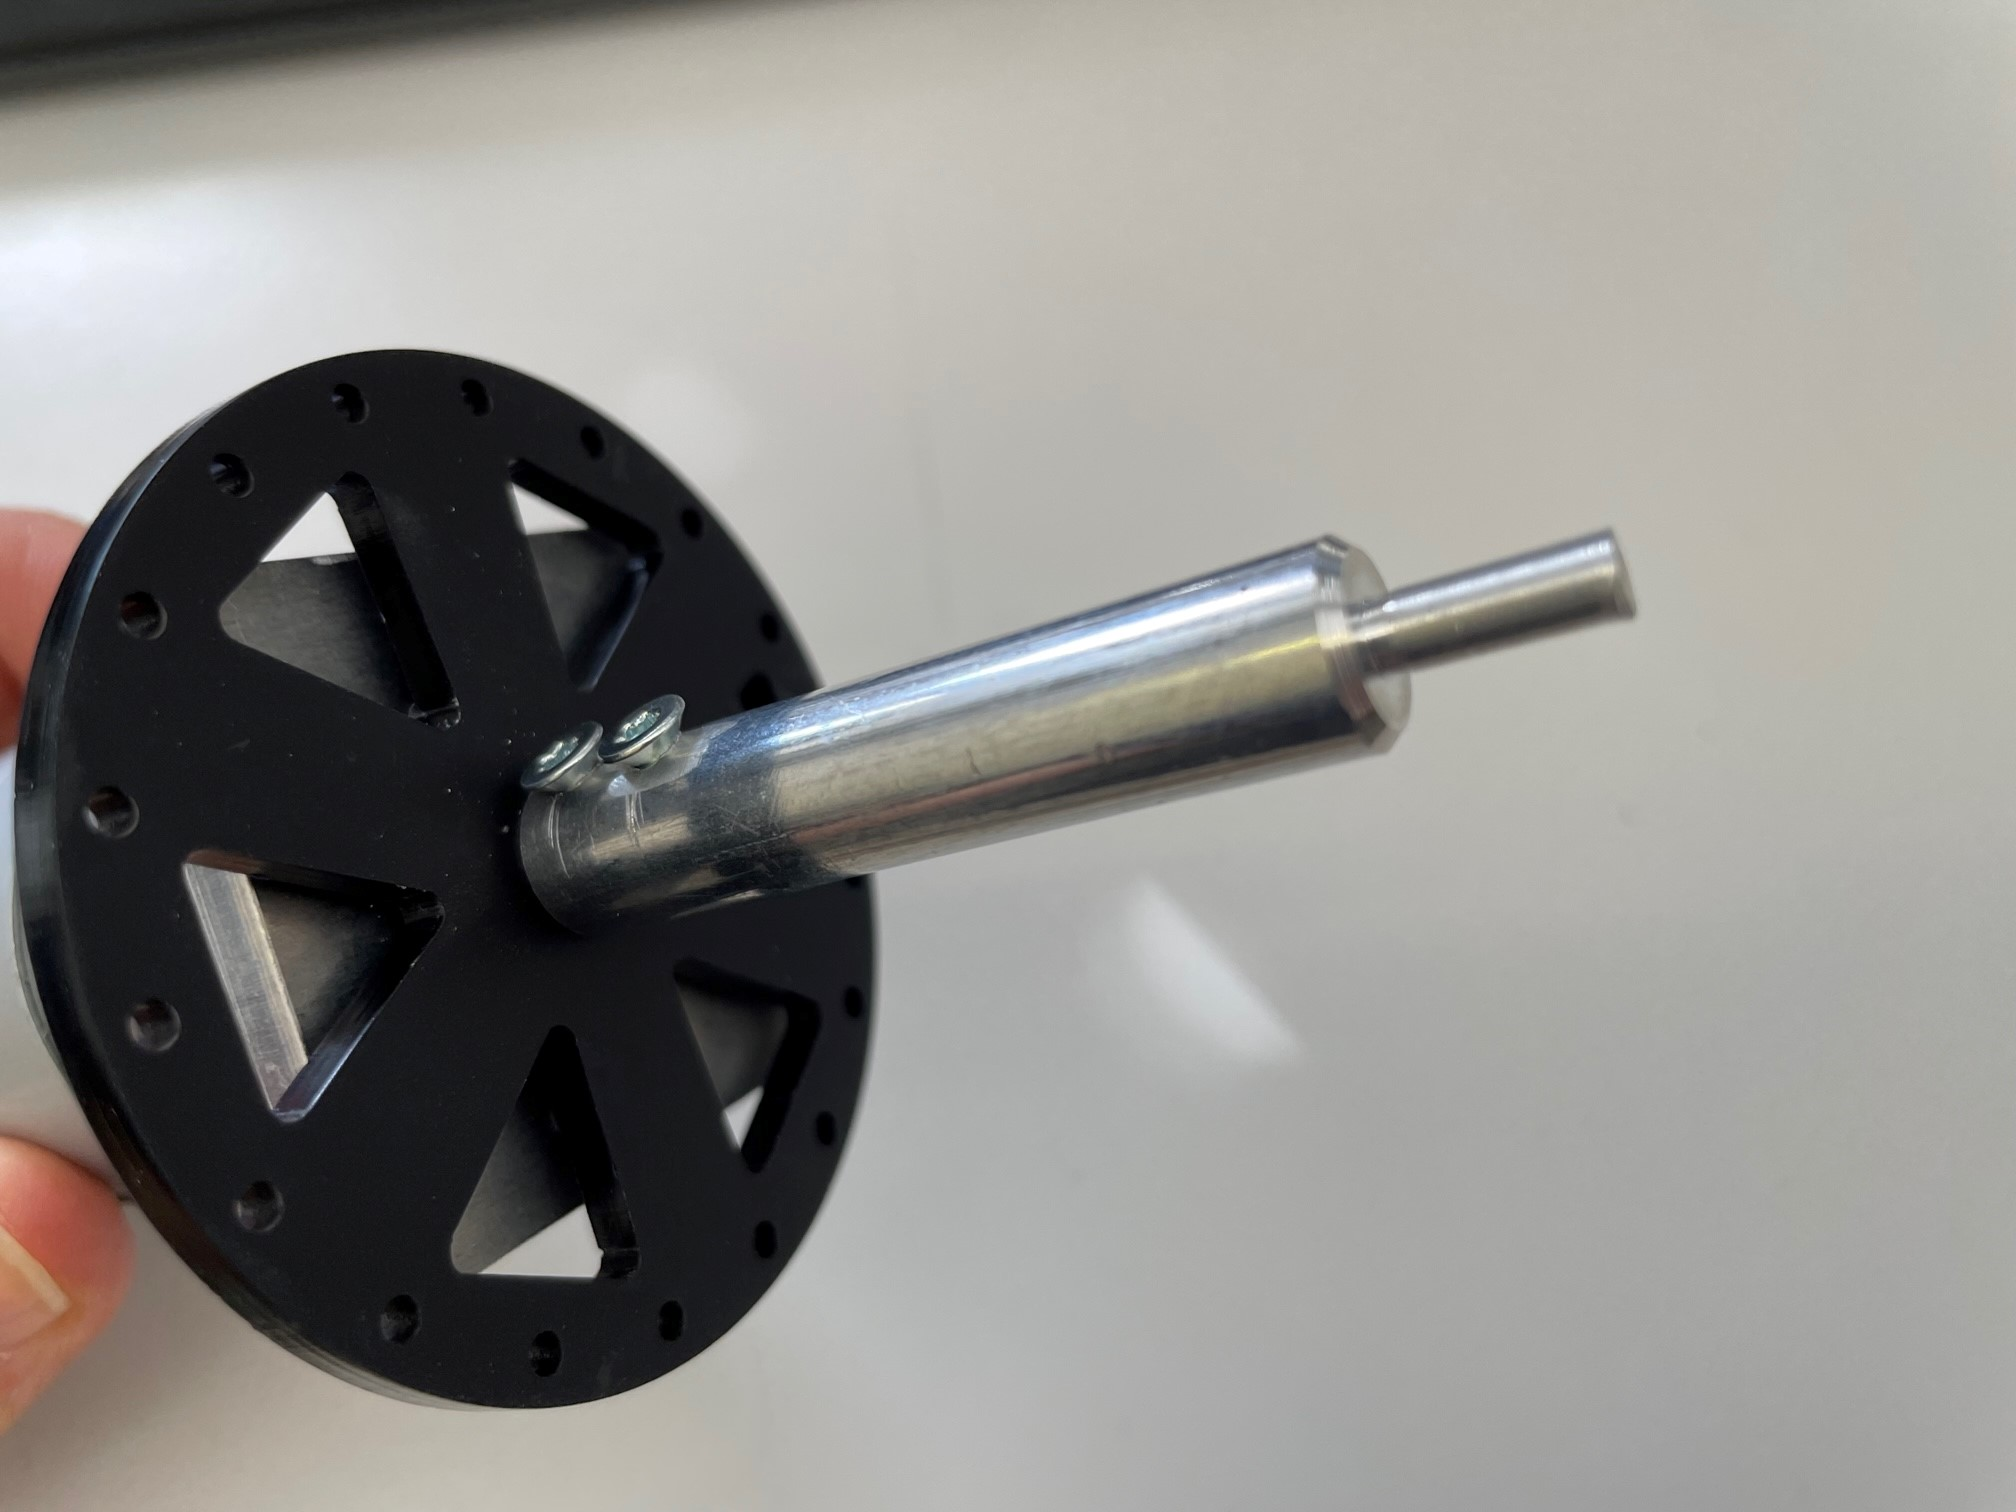
\includegraphics[scale=.1]{img/ExtensionArbreMoteur.jpg}
	\label{ExtensionRound}
	\caption{Extension d'arbre moteur ronde}
\end{figure}

La première tentative a été celle qu'on peut voir ci-dessus. L'extension était ronde avec un embout 
plus fin. Pour intégrer les roues cela n'était pas stable. Nous nous sommes alors dirigé vers une extension
hexagonale. En effet, les roues possèdent d'un côté une chambre hexagonale permettant l'insertion de l'extension. \par

\begin{figure}[!h]
	\centering 
	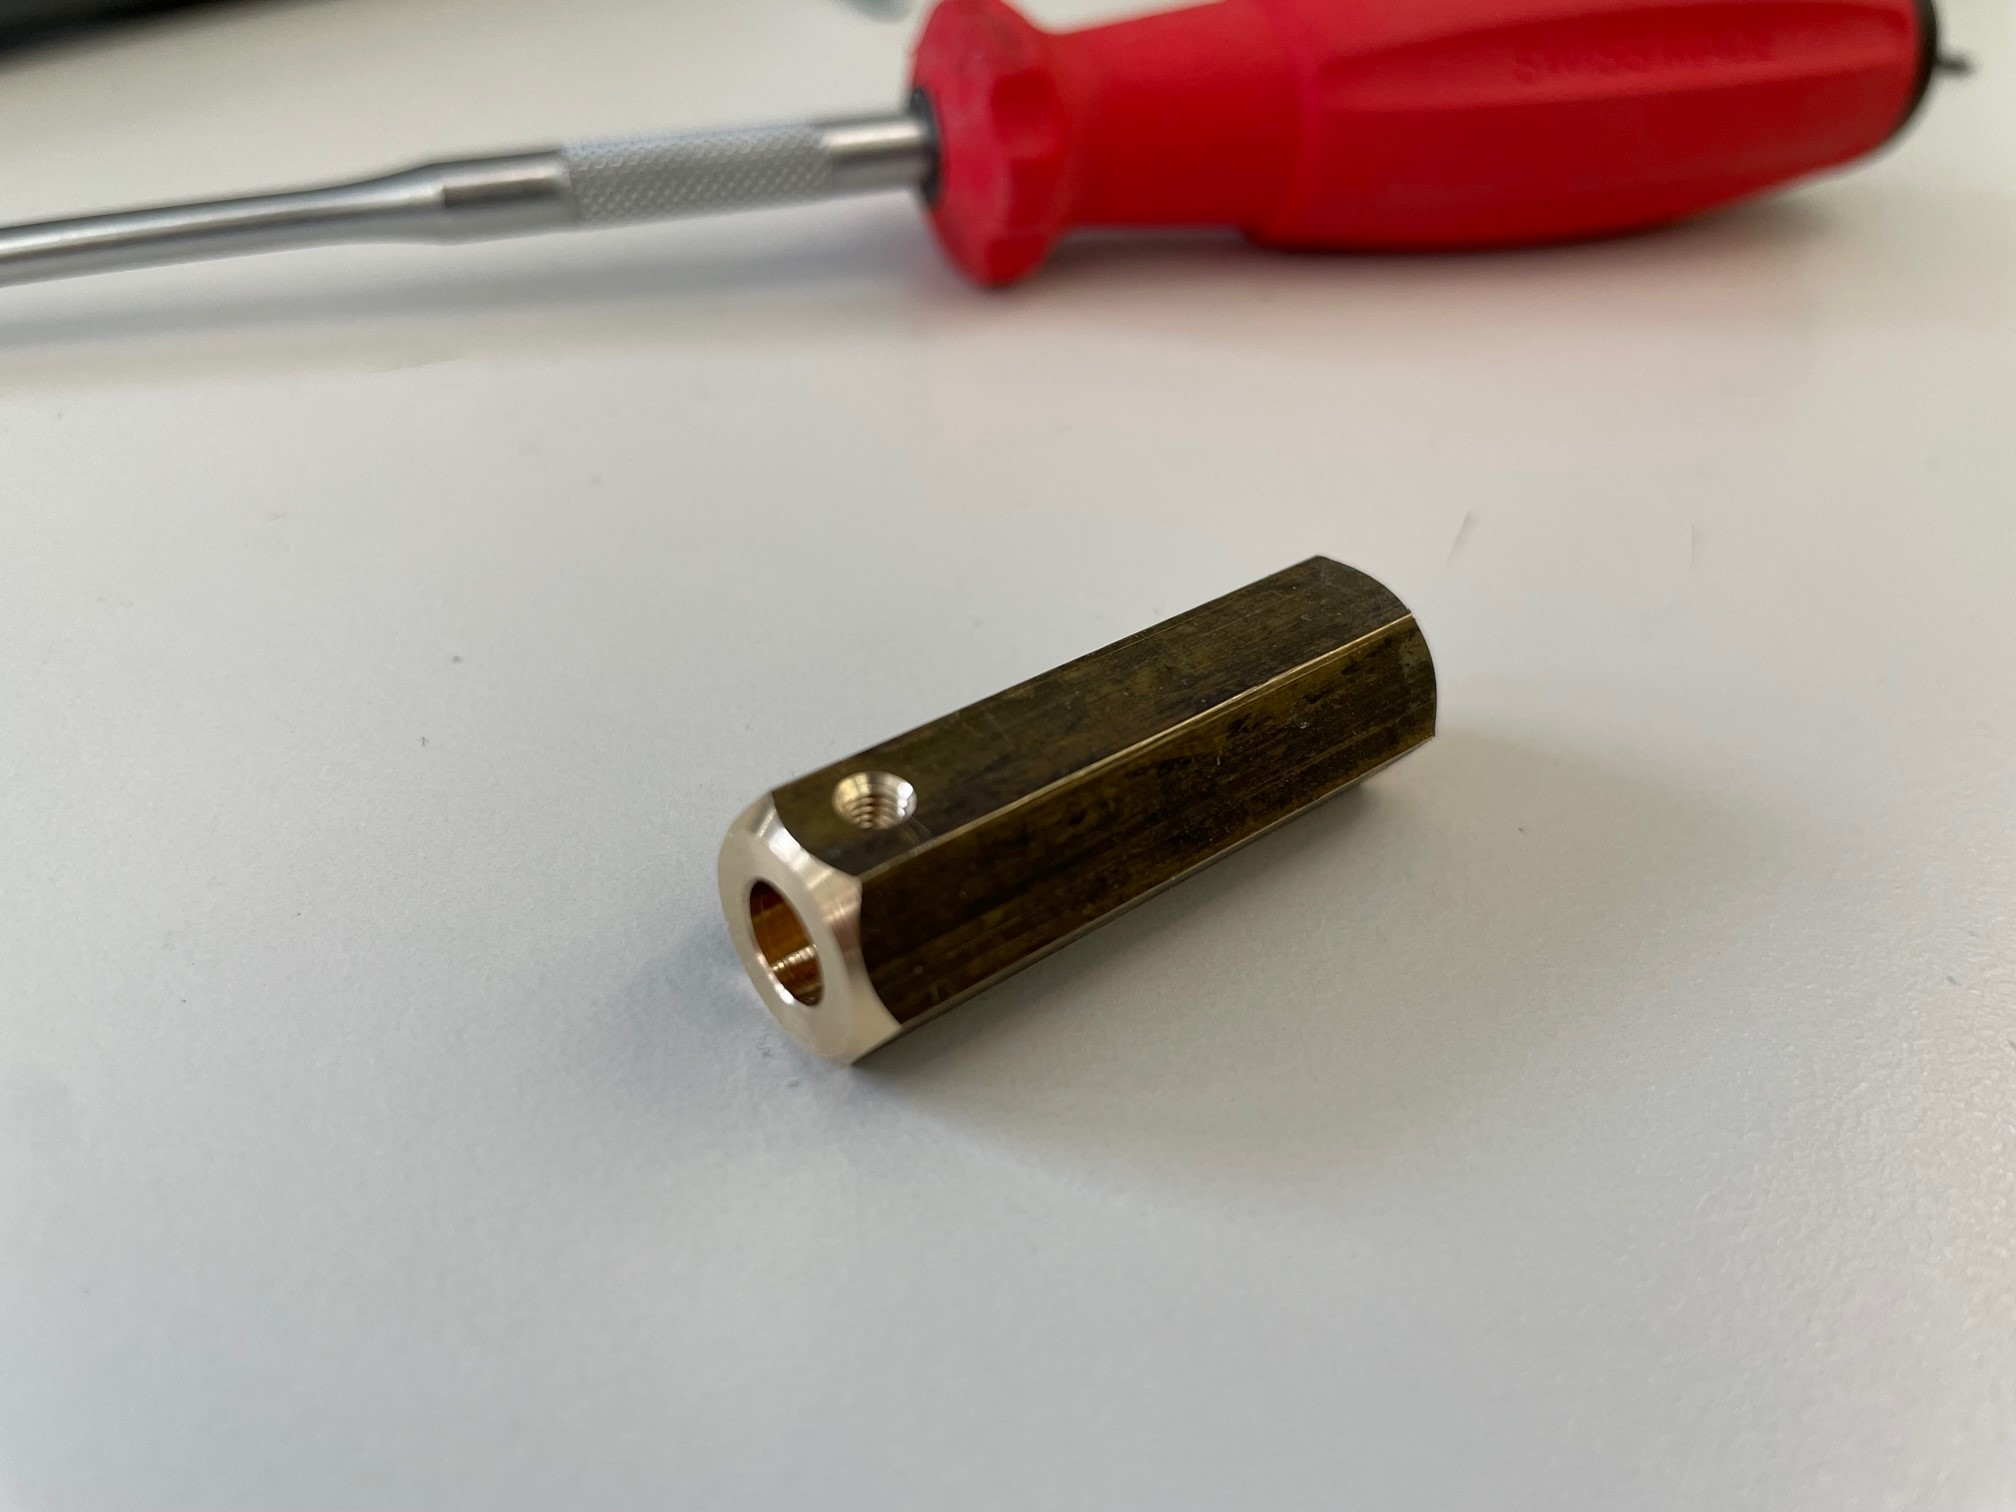
\includegraphics[scale=.1]{img/ExtensionArbreMoteurHexa.jpg}
	\label{ExtensionHexa}
	\caption{Extension d'arbre moteur hexagonale}	
\end{figure}

\newpage
L'extension hexagonale s'intègre correctement dans nos roues. Elle est facilement usinable avec la bonne pince. \par

\begin{table}[!ht]
    \begin{center}
        \vspace{5mm}
        \label{tab:table2}
        \begin{tabular}{c|c|r} % <-- Alignments: 1st column left, 2nd middle and 3rd right, with vertical lines in between
            \toprule
            \textbf{ } & \textbf{Extension Ronde} & \textbf{Extension Hexagonale}\\
            \midrule
            Temps d'usinage & 5 & 8\\
            Compatibilité & 5 & 10\\
            Maintien & 8 & 8 \\
			\midrule
			Total & 18 & 26\\
            \bottomrule
        \end{tabular}
    \end{center}    
	\caption{Comparaison des différentes extensions, échelle 1 à 10 (1 le moins bon, 10 le meilleur)}
\end{table}


Ce tableau nous permet de voir les avantages offerts par l'extension hexagonale. Cela est pourquoi nous avons 
choisi de continuer avec des extension hexagonales. 

\newpage
\section{Roues compteuses}

Nous avons faits plusieurs itérations pour les roues compteuses. Ces itérations sont intriquement liées au 
changement dans le code du PID. Nos roues compteuses ont toujours fait le même diamètre, 45mm, mais le nombre
de trous les composant a changé avec le temps. 

\begin{figure}[!h]
	\centering
	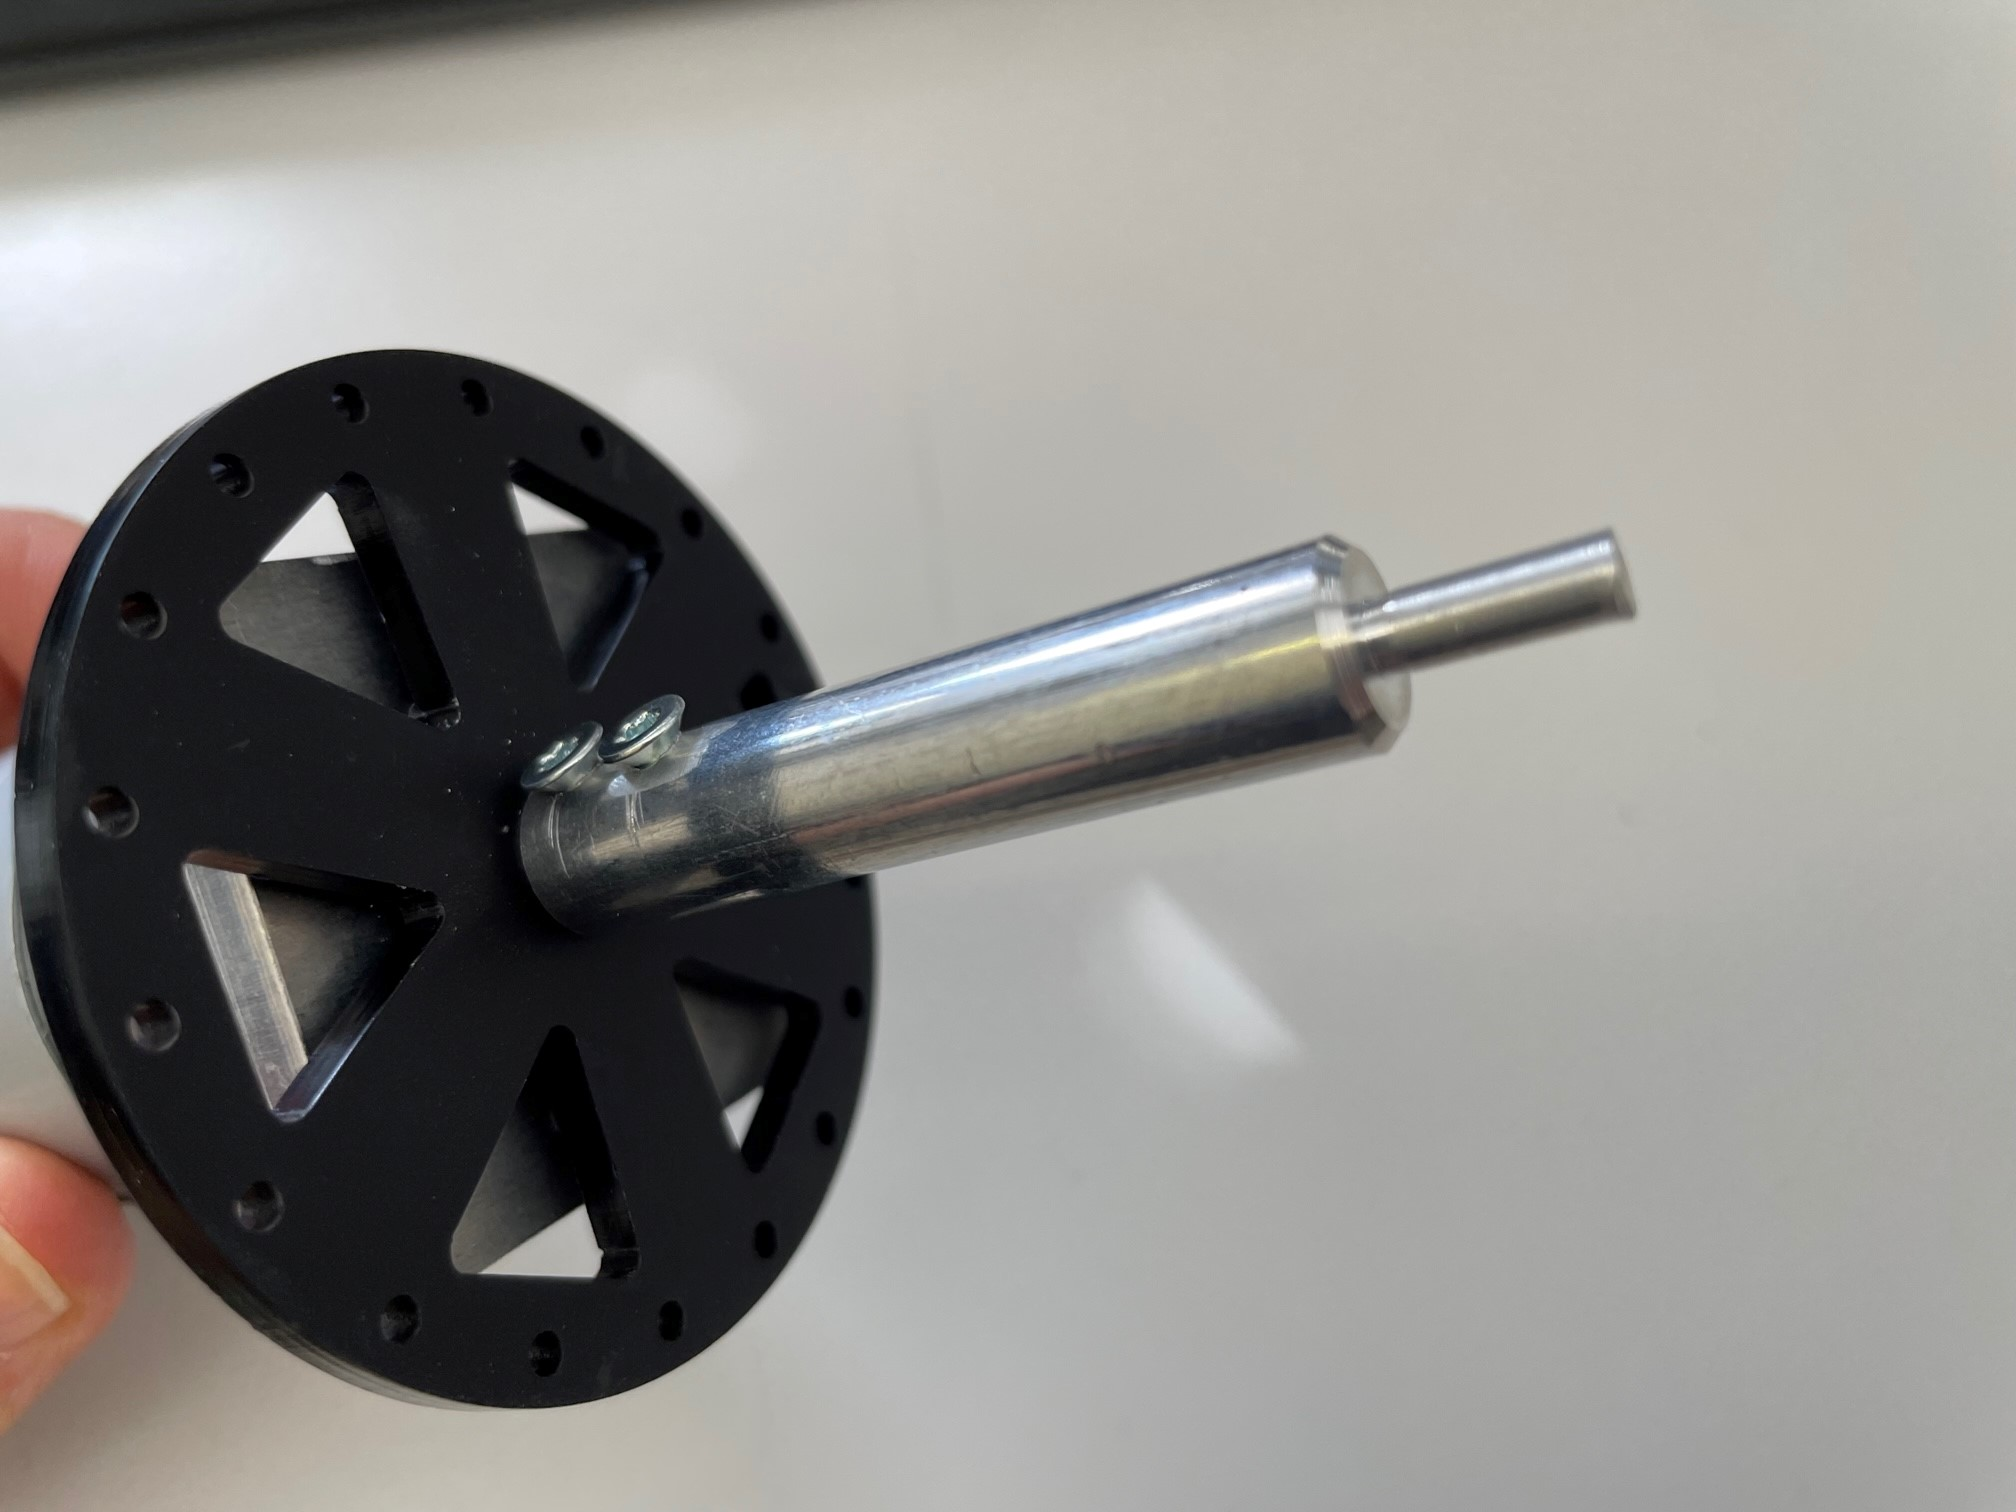
\includegraphics[scale=.1]{img/ExtensionArbreMoteur.jpg}
	\label{RoueCompteuse}
	\caption{Roue compteuse avec 16 trous}
\end{figure}

Nous voyons notre roue compteuse avec 16 trous. Nous avons une autre version avec 24 trous. La voici : 

\begin{figure}[!h]
	\centering
	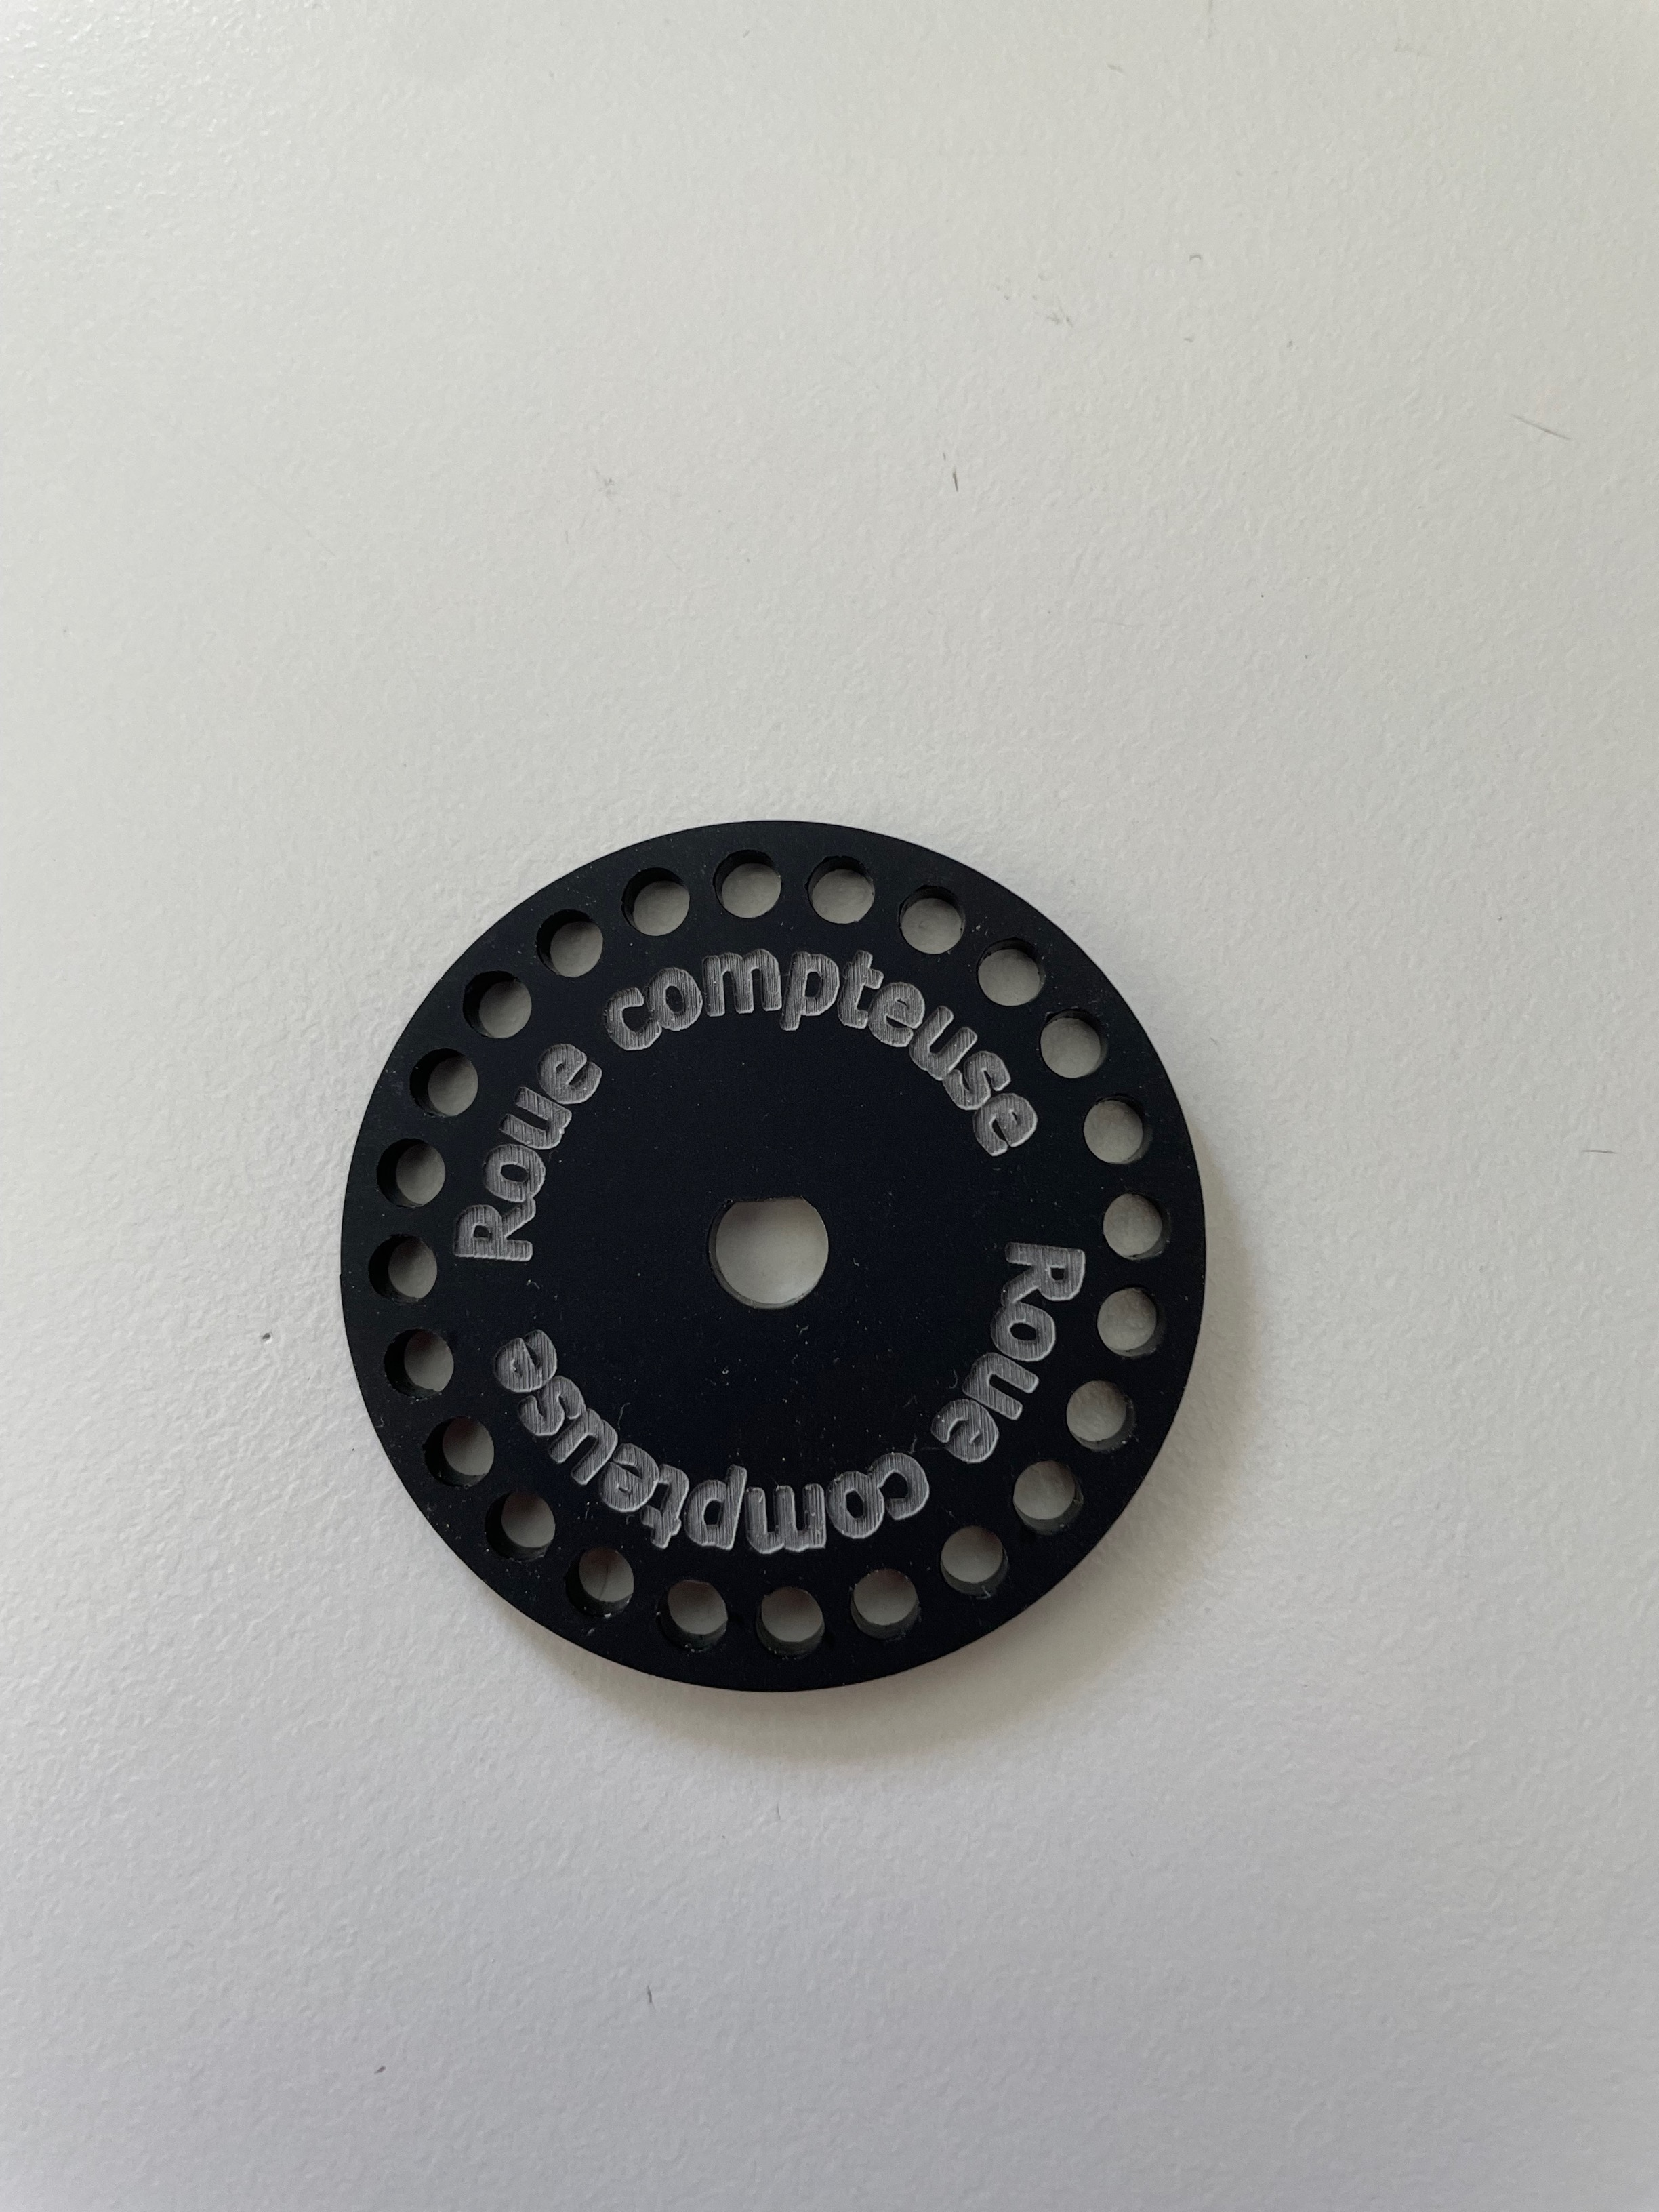
\includegraphics[scale=.08]{img/RoueCompteuse.png}
	\label{RoueCompteuse2}
	\caption{Roue compteuse avec 24 trous}
\end{figure}

Nous avons choisi la variante avec 24 trous, car c'est celle qui fonctionne le mieux avec notre code du PID.
Elle permet d'avoir, même lorsque le calcul du PID se fait à haute fréquence, d'avoir au moins une incrémentation
entre deux calculs. \par

\section{Plaque de Fondation}

Notre plaque de support, appelée "Foundation", a subi plusieurs itérations. La première les moteurs étaient en dessous
et le pont H et les batteries en dessus. Maintenant, les moteurs, les batteries et le pont H sont au-dessus. 
Cela permet de protéger les composants d'un choc avec un obstacle. \par

\begin{figure}[!ht]
	\centering 
	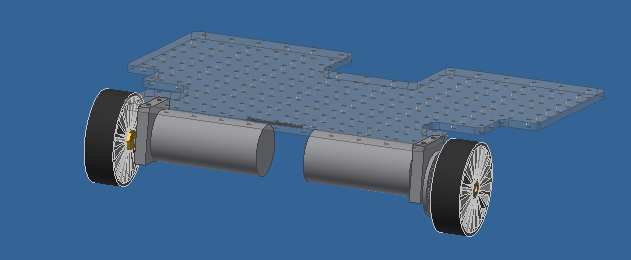
\includegraphics[scale=.5]{img/FoundationV0.png}
	\label{FoundationV0}
	\caption{Première itération "Foundation"}	
\end{figure}

Ici, nous pouvons voir la première version de notre plaque fondation. Les moteurs étaient en dessous tout comme 
les capteurs pour les roues compteuses. Cela ne garantit par leur intégrité lors du fonctionnement. \par

\begin{figure}[!ht]
	\centering 
	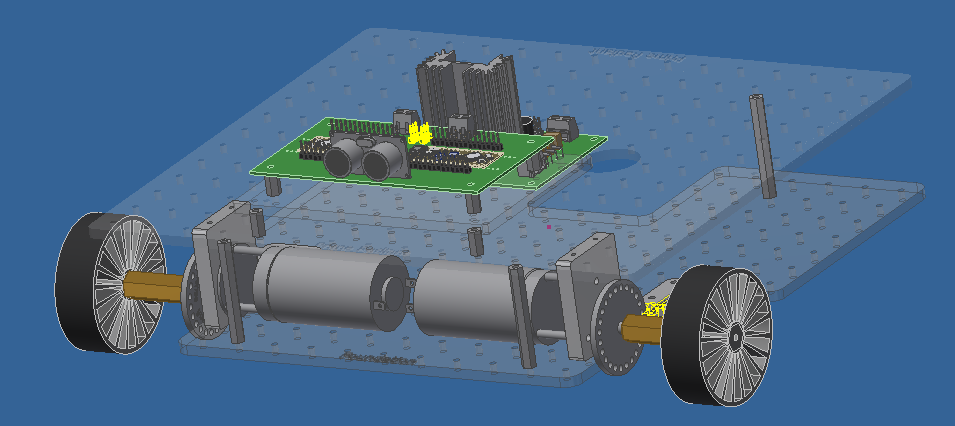
\includegraphics[scale=.4]{img/FoundationV2.0.png}
	\label{FoundationV2}
	\caption{Deuxième itération "Foundation"}	
\end{figure}

Ci-dessus, nous avons la deuxième version de la plaque "Foundation". Cette-fois ci les composants sont en-dessus
et seules les roues ont une partie qui touche le sol en dessous de la plaque.


\begin{table}[!ht]
    \begin{center}
        \vspace{5mm}
        \label{tab:table4}
        \begin{tabular}{c|c|r} % <-- Alignments: 1st column left, 2nd middle and 3rd right, with vertical lines in between
            \toprule
            \textbf{ } & \textbf{Plaque avec moteurs dessous} & \textbf{Plaque avec moteurs en dessus}\\
            \midrule
            Protection & 5 & 8\\
            Maintien des composants & 5 & 10\\
            Répartition du poids & 3 & 8 \\
			\midrule
			Total & 13 & 26\\
            \bottomrule
        \end{tabular}
    \end{center}    
	\caption{Comparaison des différentes plaques de fondation, échelle 1 à 10 (1 le moins bon, 10 le meilleur)}
\end{table}

Nous pouvons voir que la deuxième version remplit mieux nos critères. Principalement par le fait que les éléments
sont protégés des obstacles externes. La répartition du poids est aussi meilleure, tous les éléments lourds sont
le plus bas possible. \par

\section{Support Caméra}

Le support pour la caméra possède plusieurs contraintes importantes. La caméra doit vibrer le moins possible
pour avoir une qualité d'image suffisante pour pouvoir la traiter. Nous avons besoin d'une pièce robuste qui 
pourra répondre aux différentes contraintes que le support possède. \par

\begin{figure}[!h]
	\centering 
	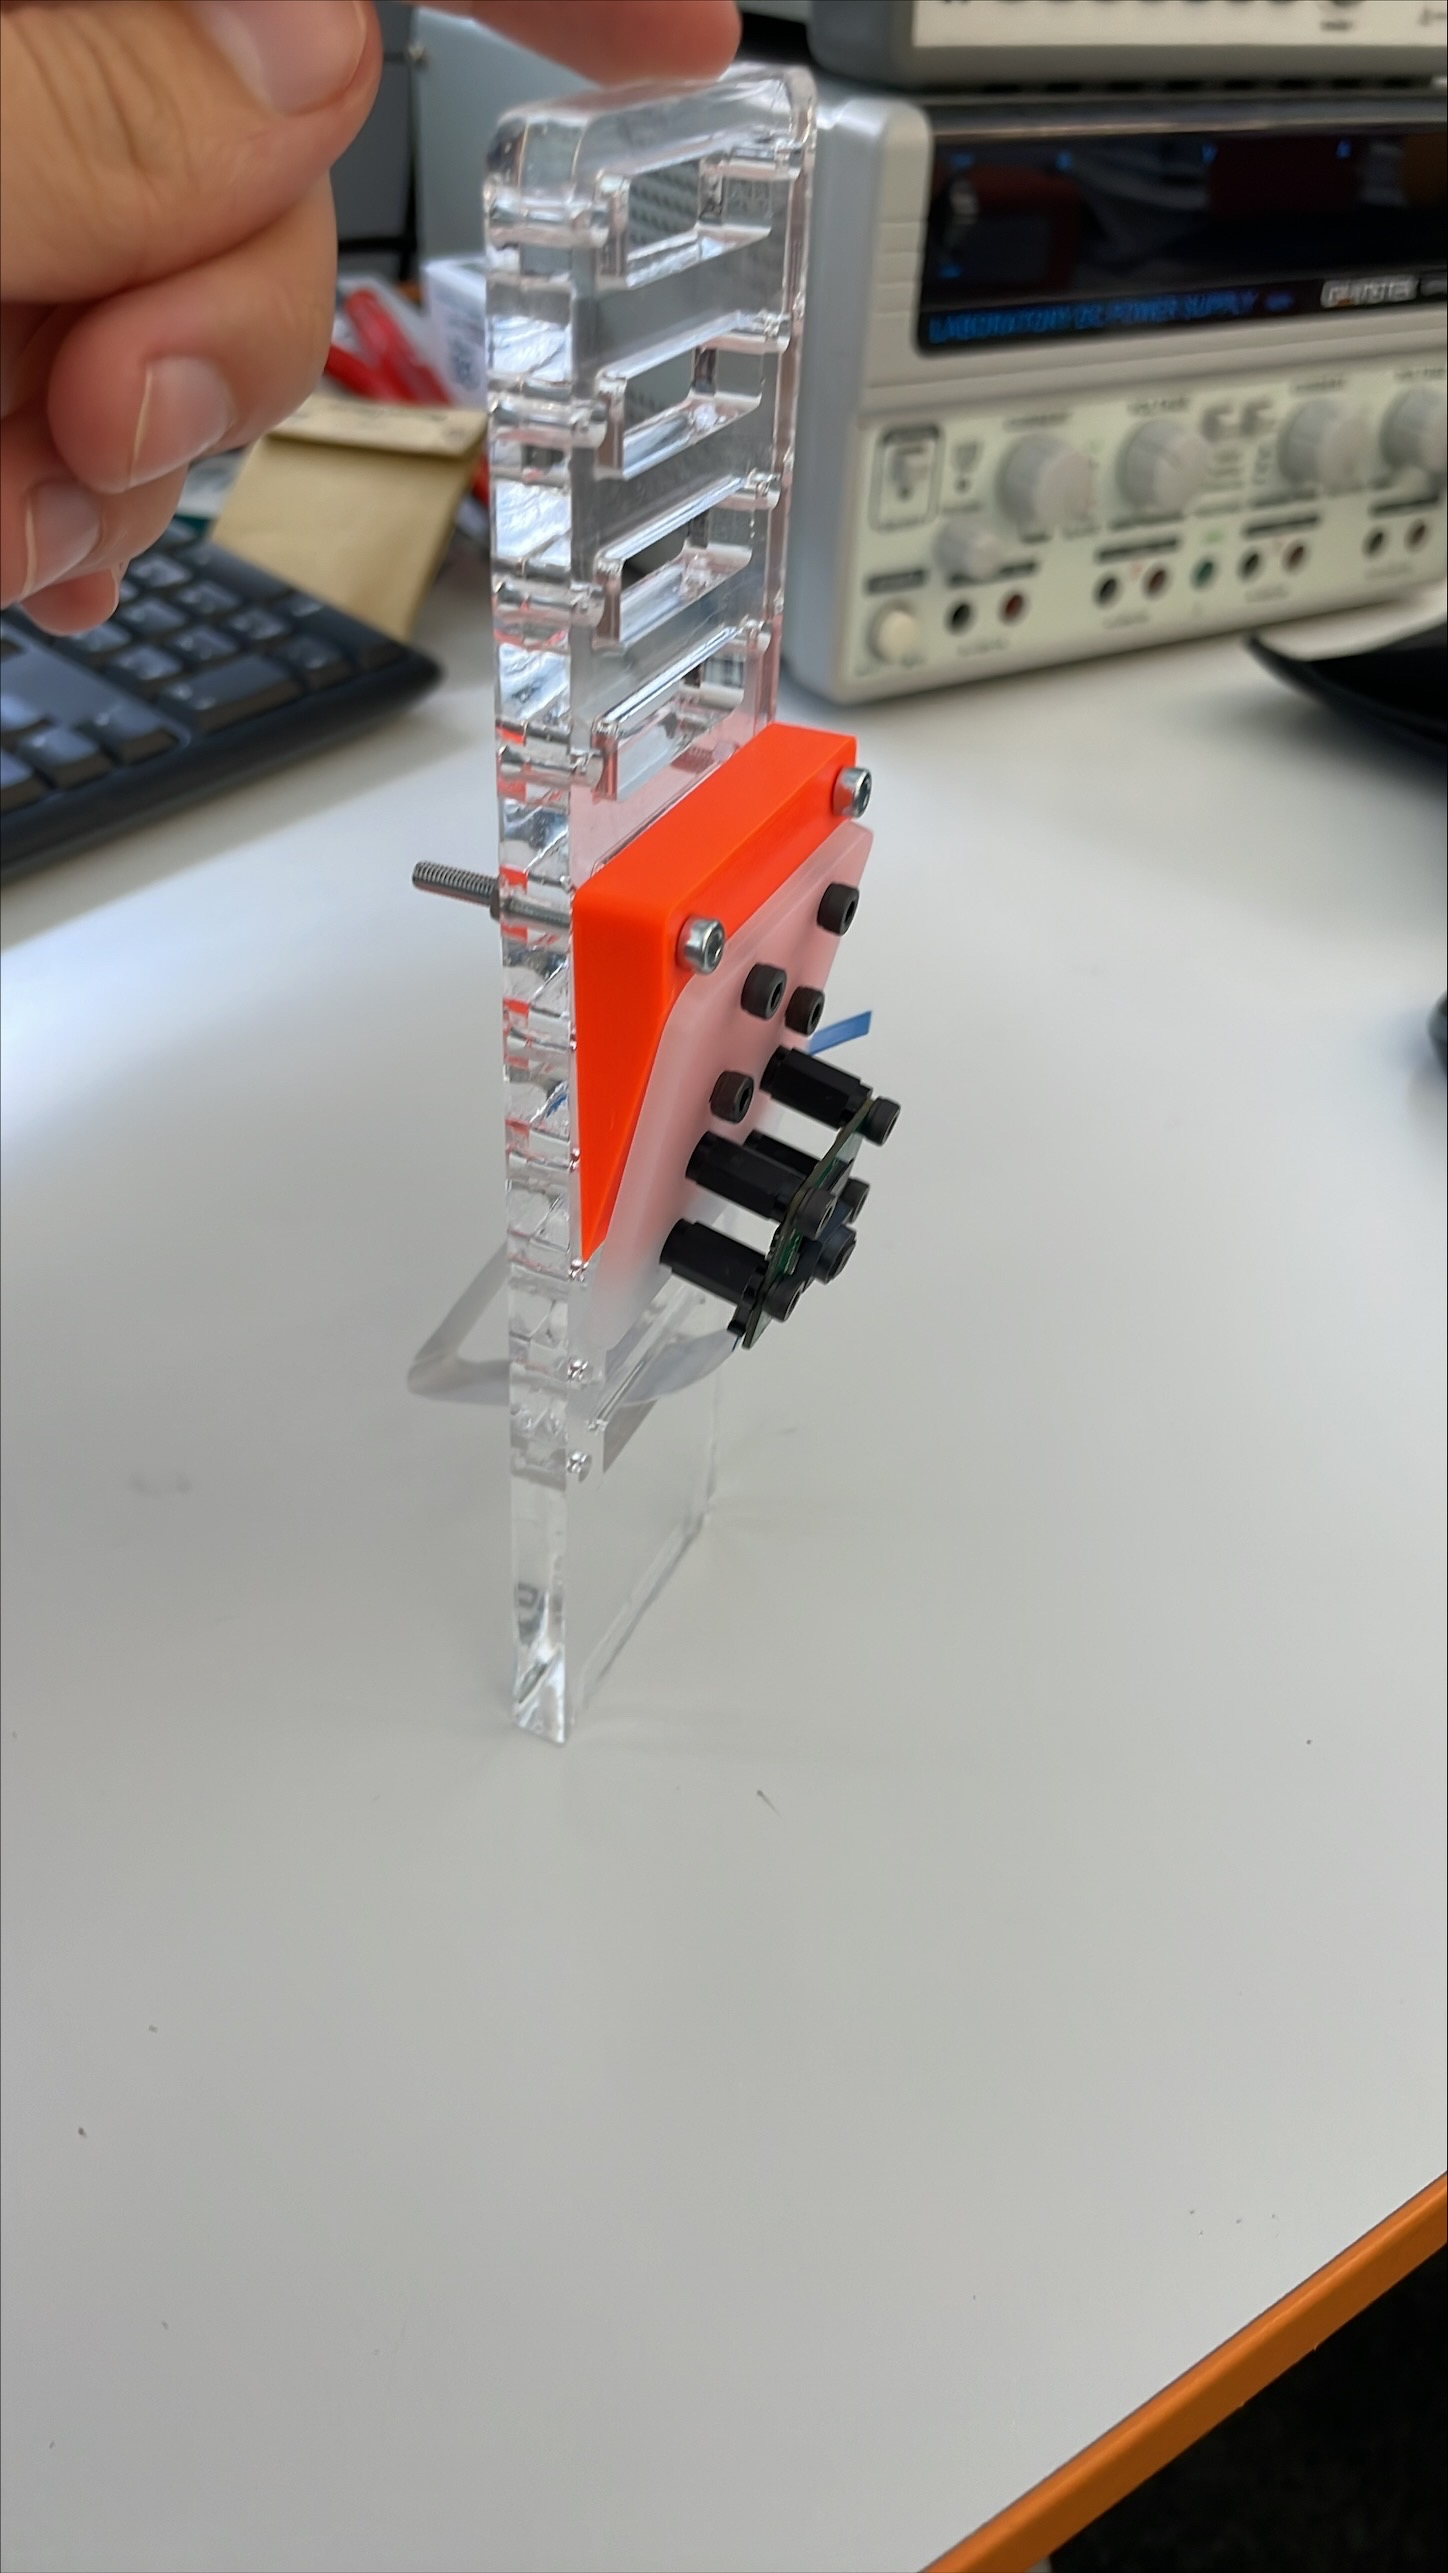
\includegraphics[scale=.1]{img/SupportCameraPI.png}
	\label{SupportCameraPI}
	\caption{Support CameraPI}	
\end{figure}

Nous pouvons voir ici une première pièce. Cependant, elle est longue. Donc plus propice à bouger par les vibrations. 
Le module pour fixer la caméra est ajouté sur l'échelle et cela peut créer des vibrations supplémentaires. \par

Nous avons donc décidé de la faire plus courte et d'une seule pièce pour éliminer ces sources de transfert de vibrations. 
Pour ce faire nous avons envoyé à l'imprimante 3D. \par

\begin{figure}[!h]
	\centering 
	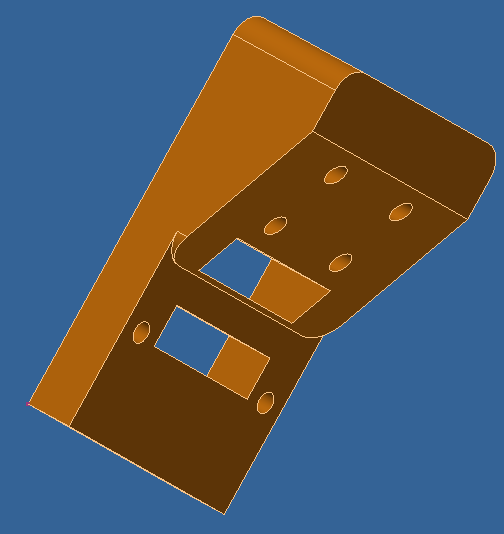
\includegraphics[scale=.4]{img/SupportCameraPIV2.png}
	\label{SupportCameraPIV2}
	\caption{Support CameraPI V2 3D}	
\end{figure}

Les contraintes ont changé le développement de la pièce pour qu'elle s'y adapte. Nous avons donc décidé de 
la fusionner en une pièce et de l'imprimer en 3D. \par



\chapter{Électronique}




1. Exposition de nos PCBs et schéma électrique ??? Est-ce qu'on doit en faire un ???
2. Argumentation de nos choix de PCBs
3. Approche des problèmes et méthodologies utilisées

\chapter{Informatique}




1. Masse de choses à dire mais être hyyyyyper clair et concis. 
2. Schéma Schéma Schéma pour qui communique quoi par quel protocole et à qui 
3. Argumentation des choix effectués pour la méthodo utilisée pour PID
4. Comprendre notre approche de la comm avec le Raspberry PI

\chapter{Améliorations}

1. Câblage et connectique du robot
2. Optimisation du code caméra pour gérer mieux le webstreaming ?
3. Opti du code de régulation du robot
4. Meilleure mécanique

\chapter{Conclusion}



\end{document}